\documentclass{beamer}
\usetheme{Warsaw}
\usepackage{nhtvslides}
\usepackage{graphicx}
\usepackage{listings}
\lstset{language=CAML,
basicstyle=\ttfamily\footnotesize,
frame=shadowbox,
breaklines=true}
\usepackage[utf8]{inputenc}

\title{Basic concepts from physics}

\author{Dr. Giuseppe Maggiore}

\institute{NHTV University of Applied Sciences \\ 
Breda, Netherlands}

\date{}

\begin{document}
\maketitle

\begin{frame}{Table of contents}
\tableofcontents
\end{frame}

\section{Body kinematics}
\begin{slide}{Introduction}{Kinematics}{
\item Study of motion
\item \textit{Position}, \textit{Velocity}, and \textit{Acceleration}
\item \textit{Rotation}, \textit{Angular velocity}, and \textit{Torque}
\item Cartesian coordinates in 2D and in 3D
}\end{slide}

\begin{slide}{Introduction}{Forces}{
\item Newton's laws of motion
}\end{slide}

\begin{slide}{Introduction}{Momenta}{
\item Linear momentum
\item Angular momentum
}\end{slide}

\begin{slide}{Introduction}{Angular momentum}{
\item Center of mass
\item Inertia tensor
\item Torque
}\end{slide}

\begin{slide}{Particle kinematics}{XY particle}{
\item We start with a particle moving across the $xy$ plane
\item Position at time $t$ is $r(t) = (x(t),y(t))$ %x(t)\iota + y(t)\jmath$ where $\iota=(1,0), \jmath=(0,1)$
%\begin{itemize}
%\item (or $(x(t),y(t))$ in tupled version)
%\end{itemize}
}\end{slide}

\begin{slide}{Particle kinematics}{XY particle}{
\item Velocity at time $t$ is $v(t) = \dot r = (\dot x,\dot y)$ \footnote{a dot above denotes derivation over time; this means that $\dot x = \frac{dx}{dt}$}
\item Speed is $|v|$
\item Acceleration is $a(t) = \dot v = \ddot r  = (\ddot x, \ddot y)$
}\end{slide}

\begin{slide}{Particle kinematics}{XY particle}{
\item Tangent is $T(t) = \frac{v}{|v|}$ % = (\cos(\phi(t)),\sin(\phi(t)))$ \footnote{$\phi = atan \frac{v_y}{v_x}$}
\item Normal is $N(t)$ and is perpendicular to $T$ % = (-\sin(\phi(t)),\cos(\phi(t)))$
\item $r,T,N$ is the \textit{moving frame} of the particle (or body space, or local space)
}\end{slide}

\begin{slide}{Particle kinematics}{XY particle motion with respect to frame}{
\item $v = |v|T = \dot s T$
\item $a = \dot v =$ % \frac{d}{dt}(\dot s T) = \ddot s T + \dot s \frac{dT}{dt} = \ddot s T + \dot s^2 \frac{dT}{ds}$ \footnote{The last step is obtained by multiplying by $\frac{ds}{dt}\frac{dt}{ds}$}
%\item Since $\frac{dT}{ds} = \frac{d\phi}{ds}N$, the acceleration is therefore $a = \ddot s T + \dot s^2 \frac{d\phi}{ds}N$
%\begin{itemize}
%\item $\ddot s T$ is the \textit{tangential acceleration}
%\item $\dot s^2 \frac{d\phi}{ds}N$ is the \textit{centripetal} (\textit{normal}) acceleration perpendicular to the direction of motion
%\end{itemize}
}\end{slide}

\begin{slide}{Particle kinematics}{XYZ particle}{
\item We now consider a particle moving in space
\item Position at time $t$ is $r(t) = (x(t),y(t),z(t))$ %where $\iota=(1,0,0), \jmath=(0,1,0), \ell=(0,0,1)$
%\begin{itemize}
%\item (or $(x(t),y(t),z(t))$ in tupled version)
%\end{itemize}
}\end{slide}

\begin{slide}{Particle kinematics}{XYZ particle}{
\item Velocity at time $t$ is $v(t) = \dot r = (\dot x, \dot y, \dot z)$
\item Speed is $|v|$
\item Acceleration is $a(t) = \dot v = \ddot r  = (\ddot x, \ddot y, \ddot z)$
}\end{slide}

\begin{slide}{Particle kinematics}{XYZ particle}{
\item Tangent is $T(t) = \frac{v}{|v|}$
\item We have an infinite set of possible vectors normal to $T$
}\end{slide}

\begin{frame}{SLIDE}
\center
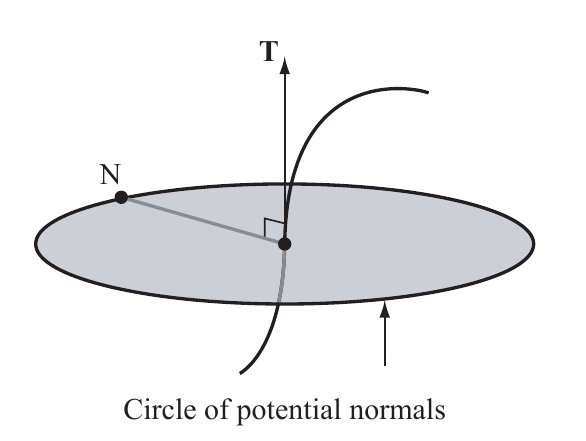
\includegraphics[width=5cm]{Pics/Fig2_3.png}
\end{frame}

\begin{slide}{Particle kinematics}{XYZ particle}{
\item Normal $N$ is perpendicular to $T$
\item We are missing an axis to have a complete frame
\item Binormal is $B = T \times N$
%\begin{itemize}
%\item $\frac{dB}{ds} = -\tau N$
%\item $\tau$ is the \textit{torsion} of the curve
%\item tendency of the curve to bend out of the $TN$ plane
%\end{itemize}
\item $r,T,N,B$ is the \textit{moving frame} of the particle (or body space, or local space)
}\end{slide}

\begin{slide}{Body kinematics}{Rigid body}{
\item $R = \left[ T\ N\ B \right] $ put in matrix form ($T, N, B$ are used as \textit{columns} of the matrix) is the \textit{rotation matrix} of the body
\item $r(t) = R(t)r_0 + x(t)$ where $x(t)$ is the position of the \textit{center} of the body
\item $\omega(t)$, a vector, is the angular velocity of the body
\begin{itemize}
\item Its direction $\frac{\omega(t)}{|\omega(t)|}$ is the rotation axis
\item Its magnitude $|\omega(t)|$ is in $rad/s$
\end{itemize}
}\end{slide}

\begin{slide}{Particle kinematics}{Rigid body rotation}{
\item We need to study $\dot r(t)$, in order to determine $\dot R$
\item We decompose $r(t)$ into $a,b$ where $a$ is parallel to $\omega$ and $b$ is perpendicular
\begin{itemize}
\item linearly moving component
\item rotating component
\end{itemize}
\item The instantaneous velocity of $r(t)$ is $\dot r = \omega(t) \times b = \omega(t) \times (a+b) = \omega(t) \times r(t)$
}\end{slide}

% PIC

\begin{slide}{Particle kinematics}{Rigid body rotation}{
\item We now consider the inertial frames, which are the columns of the rotation matrix
\item We compute $\dot T = \omega(t) \times T$, $\dot N = \omega(t) \times N$, and $\dot B = \omega(t) \times B$
\item These are the velocities of the axes of the inertial frame
\item Also known as the columns of $\dot R$
}\end{slide}

\section{Newton's laws}
\begin{slide}{Newton's laws}{Topic}{
\item Inertia, the tendency of an object to remain in motion
\item Force, the mechanism through which inertia is changed
}\end{slide}

%\begin{textslide}{Newton's laws}{First law}{
%In the absence of external forces, an object at rest will remain at rest. If the object is in motion and no external forces act on it, the object remains in motion with constant velocity. (Only forces can change an object’s motion.) 
%}\end{textslide}

%\begin{textslide}{Newton's laws}{Second law}{
%For an object of constant mass over time, its acceleration a is proportional to the force $F$ and inversely proportional to the mass $m$ of the object: $a=\frac{F}{m}$. We normally see this written as $F=ma$. If the mass changes over time, the more general statement of the law is $F=\frac{d}{dt}(mv) + \frac{dm}{dt}v$, where $v$ is the velocity of the object. The quantity $mv$ is the linear momentum of the object. Thus, the second law states that the application of an external force on an object causes a change in the object's momentum over time. (An object's path of motion is determined from the applied forces.)
%}\end{textslide}

%\begin{textslide}{Newton's laws}{Third law}{
%If a force is exerted on one object, there is a force of equal magnitude but opposite direction on some other body that interacts with it. (Action and reaction always occur between interacting objects.)
%}\end{textslide}

\begin{slide}{Newton's laws}{About the laws}{
\item The \textbf{second law} is the one we work the most with
\item Mass is assumed to be always constant, so $F=\frac{d}{dt}(mv) = m\frac{d}{dt}v = ma$
\item Each of the vector quantities of position, velocity, and acceleration is measured with respect to some arbitrary but fixed coordinate system, referred to as the \textit{inertial frame}, or global space
}\end{slide}

\section{Torque}
\begin{slide}{Torque}{From force to torque}{
\item Removing log nuts with a wrench
\item Exert a force on the end of the wrench, the nut turns
\item The longer the wrench, the easier (but slower) the nut turns
}\end{slide}

\begin{frame}{SLIDE}
\center
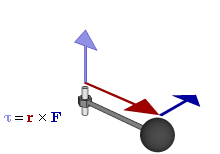
\includegraphics[width=4cm]{Pics/Torque_animation.png}
\end{frame}

\begin{slide}{Torque}{Definition}{
\item The \textit{ease} of turning is proportional to the length of the wrench and the force applied
\item This product is referred to as \textit{torque} or \textit{moment of force}
\item Torque is defined as $\tau = r \times F$
\begin{itemize}
\item Direction of torque is axis (and direction) of rotation
\item Length of torque is in $rad/s$
\end{itemize}
}\end{slide}

\begin{slide}{Torque}{Multiple torques}{
\item Multiple torques (just like forces) are simply added together
\item $\tau = \sum_i r_i \times F_i$ (discrete body) or $\tau = \int r \times F dr$ (continuous body)
}\end{slide}

\section{Momenta}
\begin{slide}{Momenta}{Momenta}{
\item Quantification of Newton's \textbf{Second Law}
\item How much \textit{motion} does the body have?
\begin{itemize}
\item \textbf{A lot} means that a lot of force is needed to change it
\item \textbf{Little} means that little force is needed to change it
\end{itemize}
}\end{slide}

\begin{slide}{Momenta}{Linear momentum}{
\item How much linear \textit{motion} does the body have?
\item $p=mv=\sum_i m_i v_i=\int_R v\ dm$
%\item Linear momentum is conserved in a system
%\begin{itemize}
%\item W.r.t. all bodies $\frac{dP}{dt} = 0$
%\end{itemize}
\item Force integrates linear momentum directly
\item $\frac{dp}{dt} = \frac{d(mv)}{dt} = m \frac{dv}{dt} = ma = F$
}\end{slide}

\begin{slide}{Momenta}{Angular momentum}{
\item How much rotational \textit{motion} does the body have?
\item $L=r \times p=m r \times v$
\item Right-hand rule of cross-product:
\begin{itemize}
\item Angular momentum refers to the tendency of the body to rotate around a given axis, $L$
\item The longer the axis, the harder it is to stop the rotation
\end{itemize}
}\end{slide}

%\begin{slide}{Momenta}{Angular momentum}{
%\item $L=\sum_i m_i r_i \times v_i=\int_R r \times v dm$
%\item Angular momentum is conserved in a system
%\begin{itemize}
%\item w.r.t. all bodies $\frac{dL}{dt} = 0$
%\end{itemize}
%}\end{slide}

\begin{slide}{Momenta}{Angular momentum}{
\item Just like the derivative of linear momentum is force...
\item ...angular momentum derived yields torque (when the body does not change shape)
\item $\frac{dL}{dp} = \tau$
%\begin{eqnarray}
%\frac{dL}{dp} &=& \frac{d r \times p}{dt} \\
%&=& r \times \frac{dp}{dt} + \frac{dr}{dt} \times p \\
%&\circeq& r \times F \\
%&=& \tau
%\end{eqnarray}
}\end{slide}

\section{Center of mass}
\begin{slide}{Center of mass}{Tracking particles?}{
\item Do we really need to track all the particles of a rigid body?
\item No!
\begin{itemize}
\item Too slow
\item \textit{Center} of mass
\item Properties of the motion \textit{of the whole body}
\item Rigid body behaves as if all the mass were concentrated at a single point
\end{itemize}
\item We compute the center of mass by a weighted average of the body particles relative positions and their respective masses
%\begin{itemize}
%\item $\sum_i m_i g (x_i - \bar x) = 0$
%\end{itemize}
}\end{slide}

\begin{slide}{Center of mass}{One dimension}{
\item A wooden plank with two \textit{weights} at the extremes
\item Center of mass is $\bar x = \frac{m_1 x_1 + m_2 x_2}{m_1 + m_2} = x_1 \frac{m_1}{m_1+m_2} + x_2 \frac{m_2}{m_1+m_2}$
}\end{slide}

\begin{frame}{SLIDE}
\center
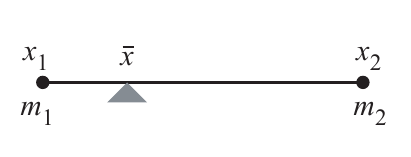
\includegraphics[width=5cm]{Pics/Fig2_15.png}
\end{frame}

%\begin{slide}{Center of mass}{One dimension}{
%\item Multiple \textit{weights} along the plank
%\item Center of mass \footnote{From now on, $M = \sum_i m_i$} is $\bar x = \frac{\sum_i m_i x_i}{M}$
%\pause
%\item For a continuous mass, replace summation with integral
%\item $\bar x = \frac{\int_l x \delta(x) dx}{\int_l delta(x) dx}$
%}\end{slide}

\begin{slide}{Center of mass}{Two dimensions}{
\item Center of mass is $\bar x = \frac{\sum_i m_i x_i}{M}$, where $x_i$ is a 2D vector \footnote{Component-wise, the result  is $(\bar x,\bar y) = (\frac{\sum_i m_i x_i}{M},\frac{\sum_i m_i y_i}{M})$}
%\pause
%\item For a continuous mass, replace summation with integral
%\item $\bar x = \frac{\int_l x \delta(x) dx}{\int_l delta(x) dx}$
}\end{slide}

\begin{slide}{Center of mass}{Three dimensions}{
\item Center of mass is $\bar x = \frac{\sum_i m_i x_i}{M}$, where $x_i$ is a 3D vector
%\pause
%\item For a continuous mass, replace summation with integral
%\item $\bar x = \frac{\int_l x \delta(x) dx}{\int_l delta(x) dx}$
}\end{slide}

\begin{slide}{Center of mass}{Force projection}{
\item When an external force $F_{\text{ext}}$ is applied to a body from some position, $r_f$
\item We use the center of mass to split the force between linear and torque
\item $F = F_{\text{ext}} \cdot \frac{(r_f - \bar x)}{|(r_f - \bar x)|}$, $\tau = F_{\text{ext}} \times (r_f - \bar x)$
}\end{slide}

\section{Moments of inertia}
\begin{slide}{Moments of inertia}{Moments of inertia}{
\item \textit{How difficult is it to set an object into rotation around an axis?}
\item Rotational equivalent to mass for linear movement
}\end{slide}

%\begin{slide}{Moments of inertia}{Moment of inertia in 1D}{
%\item The more a particle weighs, or the further from the center, the harder to set the object into rotation
%\item For the whole body we sum the contributions of each particle: $I = \sum_i m_i (x_i - \bar x)^2 = \sum_i m_i x_i^2 - m \bar x^2$
%}\end{slide}

\begin{slide}{Moments of inertia}{Moment of inertia in 2D}{
\item A single number, because in 2D we can only rotate in one plane
\item $I = \sum_i m_i |(x_i,y_i) - (\bar x, \bar y)| ^2 = \sum_i m_i (x_i^2 + y_i^2) - m(\bar x^2, \bar y^2)$
}\end{slide}

\begin{slide}{Moments of inertia}{Moment of inertia in 3D}{
\item Harder to express, because suddenly we can rotate along an infinite number of axes
\item Let us engineer this from the angular momentum of a particle of the body
\item Consider a particle 
\begin{itemize}
\item Located at relative vector $r$
\item Moving with linear velocity $v = \omega \times r$
\end{itemize}
}\end{slide}

\begin{slide}{Moments of inertia}{Mass matrix in 3D}{
\item $L_i = r_i \times m_i v_i = m_i r_i \times (\omega \times r_i) = J\omega$
\item $J_i = m_i \left[ \begin{matrix}
y_i^2 + z_i^2 & -x_iy_i & -x_iz_i \\
-x_iy_i & x_i^2 + z_i^2 & -y_iz_i \\
-x_iz_i & -y_iz_i & y_i^2 + z_i^2 \\
\end{matrix} \right] $
\item $L_i = J_i\omega$, just like $P = mv$
\item For the whole body, we sum all the $J_i$ matrices of the particles
\item $J = \sum_i J_i$, $L = J \omega$
\item $J$ must be recalculated from the rotated body, because $r_i = R r_0 + \bar x$
}\end{slide}

\section{Whole kinematics}
\begin{slide}{Whole kinematics}{Whole kinematics}{
\item Position, integrated from velocity $\dot x = v$
\item Velocity, derived from linear momentum $v = \frac{P}{m}$
\item Linear momentum, integrated from force $\dot P = F_{\text{ext}} \cdot \frac{(r_f - \bar x)}{|(r_f - \bar x)|}$
}\end{slide}

\begin{slide}{Whole kinematics}{Whole kinematics}{
\item Rotation, integrated from angular velocity $\dot R = [\omega \times T\ \omega \times N\ \omega \times B]$
\item Angular velocity, derived from angular momentum $\omega = J^{-1} L$
\item Angular momentum, integrated from torque $\dot L = \tau = \frac{(r_f - \bar x)}{|(r_f - \bar x)|} \times F_{\text{ext}}$
}\end{slide}

\begin{frame}{That's it}
\center
\fontsize{18pt}{7.2}\selectfont
Thank you!
\end{frame}

\end{document}
